\chapter{Reactor Mass Model Results}\label{ch:power_cycle_results}
The reactor mass model was tested in response to various flow inputs. This
chapter will provide some qualitative discussion about the reactor response to
coolant mass flow rate, temperature, and pressure. The most interesting response
metric was how reactor mass changed with thermal power.
In the most general sense, the reactor mass model can be described as:

\begin{equation}
    m_{reactor} = f(\dot{m}, T_{in}, T_{out}, P_{in}, P_{out})
\end{equation}

The minimum reactor mass was dependent on these flow conditions. The flow
conditions dictated the required thermal power and affected the achievable power
density of the reactor through mass flow rate (convective heat transfer) and
coolant temperature ($\Delta$ T from fuel to coolant).

\section{Reactor Response to Flow Inputs}

\subsection{Mass Flow Rate}
The mass flow rate through the core was dictated by the power cycle model. It was
the free variable used by the power cycle model to meet the required 40 kWe
output of the system. Increasing the mass flow rate improved the heat transfer
coefficient from the fuel to the coolant. Reactors with higher mass flow rates
have less resistance to convection and better cooling. While the mass flow rate
helps heat transfer in the reactor, it was also used to adjust power output. For
a fixed coolant temperature rise, increasing the mass flow rate increased the
required thermal output of the reactor. Increasing the output of the core always
increased the mass. Mass flow rate was a tradeoff between heat transfer
performance and required thermal power.

\subsection{Coolant Temperature}
Bulk coolant temperatures were used to calculate coolant properties and the
temperature drop from the fuel to coolant. Increasing the coolant temperature
decreases this temperature drop. This decrease in $\Delta$T from fuel to coolant
reduced the
achievable volumetric power density of the core, requiring a larger core volume to deliver the same
thermal power. While increasing coolant temperature reduced the thermal power
density of the reactor, it also improved the efficiency of the power cycle. A
more efficient cycle required a smaller thermal input to generate a fixed amount
of electrical power.

\subsection{Coolant Pressure}
Bulk coolant pressures were used to calculate coolant properties, Appendix
\ref{ch:appendix-b} contains property plots as a function of temperature for
various pressures. Pressure also impacted the thickness of the pressure vessel.
Higher pressure systems required a thicker pressure vessel for containment, and more mass.

\subsection{Thermal Power}
Reactor mass response to thermal power was tested at a fixed axial coolant temperature
rise across the core. Coolant mass flow rate was adjusted to match thermal power
and the fixed temperature drop. The following equation was used to determine
coolant mass flow rate.
\begin{equation}
    \dot{m} = \frac{P}{C_p \Delta T}
\end{equation}
Where C$_p$ is the coolant specific heat capacity [$\frac{kJ}{kg-K}$] and
$\Delta T$ is the axial temperature rise in the coolant.
Figure \ref{fig:mass_vs_q_uo2_co2} shows the reactor mass dependence on thermal
power.

\begin{figure}[h]
    \centering
    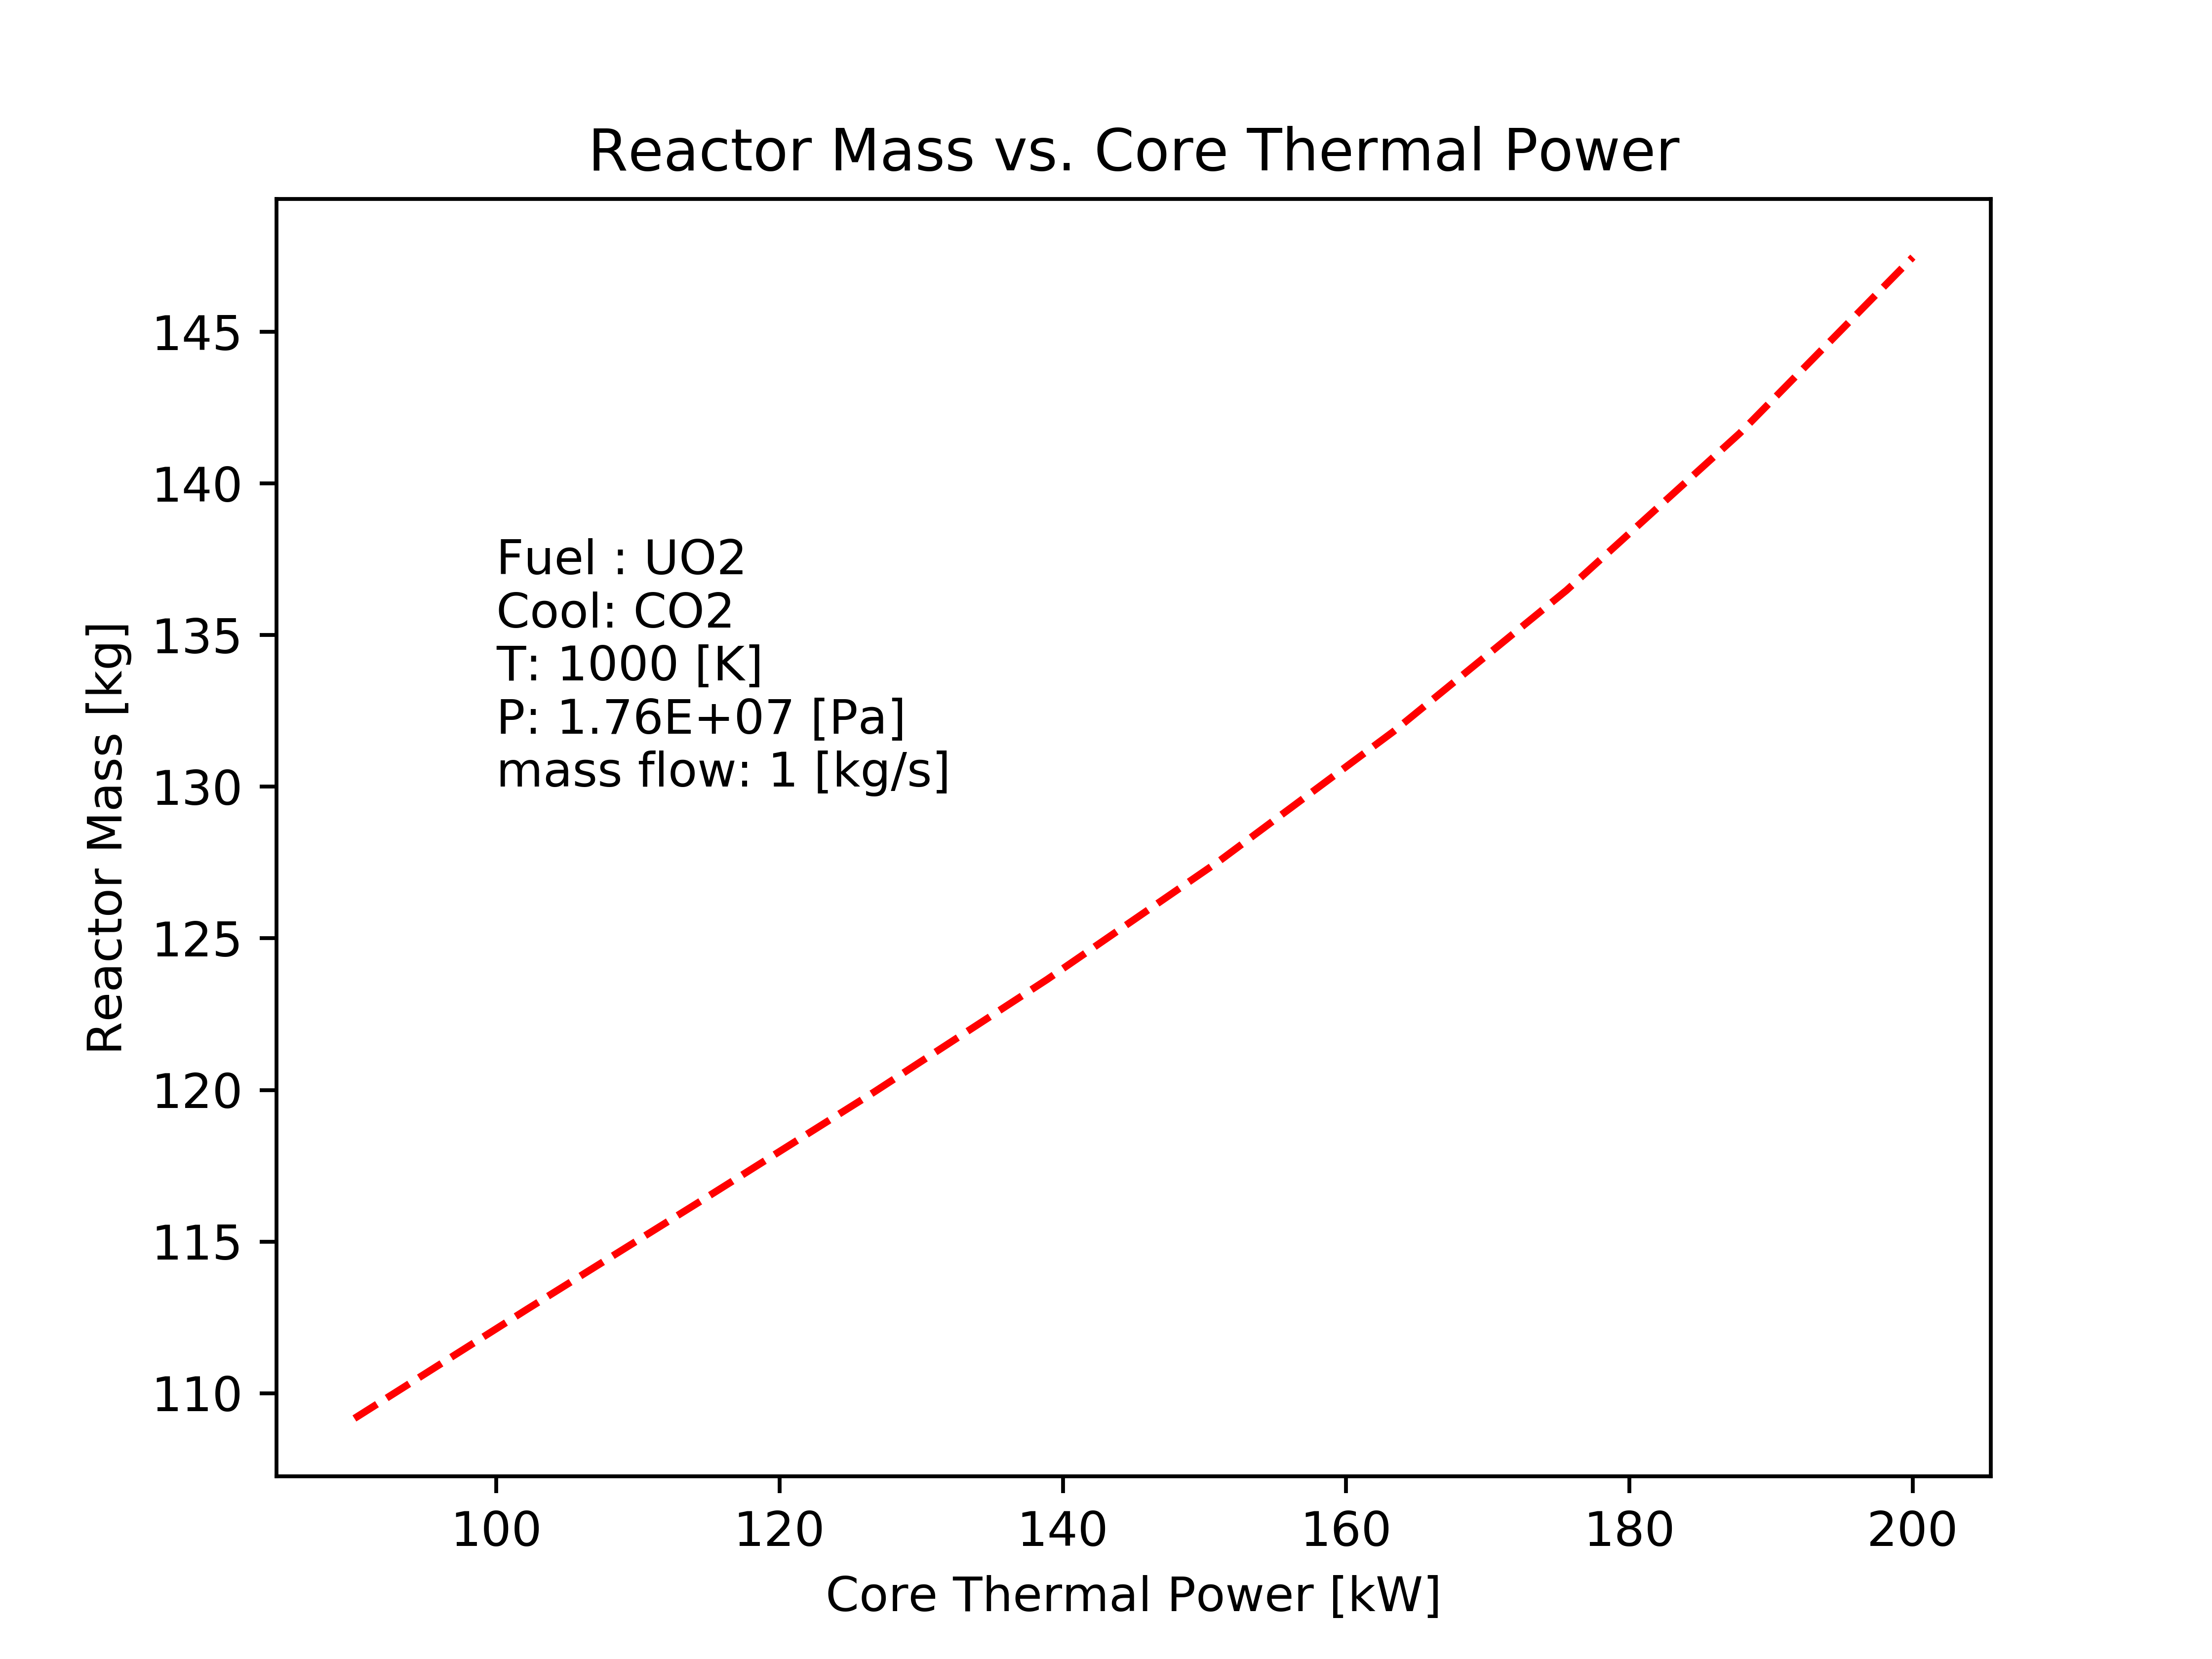
\includegraphics[width=4in]{../images/mass_vs_q_uo2_co2.png}
\caption{Reactor mass power dependence}
\label{fig:mass_vs_q_uo2_co2}
\end{figure}

\section{Reactor Mass Model Results Summary}
A reactor mass model was developed from thermal hydraulic and reactivity
requirements (discussed in \ref{ch:crit_radius}). The model solved the heat
transfer equations iteratively to return a reactor model that meets the thermal
input requirements of the power cycle. The mass model was demonstrated here for
the \uox-\codiox  reactor configuration. Three other configurations were
considered using UN-\codiox, \uox-\water, and UN-\water. The results of these
configurations, as well as their corresponding reactivity models can be found in
Appendix \ref{ch:appendix-a}.
